\documentclass[11pt,a4paper,bibtotoc,idxtotoc,headsepline,footsepline,footexclude,BCOR12mm,DIV13]{scrbook}


% Second template
% Set here the title, authors and other stuff to be used for the cover
% This file is used by MAIN.TEX

% set title, authors and stuff for the cover
\def\doctype{Master Thesis in Informatics}
\def\title{Adding C++ Support to MBEDDR}
\def\titleGer{C++ Unterst\"utzung f\"ur MBEDDR}
\def\author{Zaur Molotnikov}
\def\date{September 15, 2013}
\def\dateGer{15. September 2013}
\def\advisor{Dr. Daniel Ratiu}
\def\supervisor{Dr. Bernhard Sch\"atz}

% text to appear in the footer
\def\footertext{}
% include settings
% Included by MAIN.TEX
% Defines the settings for the CAMP report document

\renewcommand{\sectfont}{\normalfont \bfseries}        % Schriftart der Kopfzeile

% manipulate footer
\usepackage{scrpage2}
\pagestyle{scrheadings}
\ifoot[\footertext]{\footertext} % \footertext set in INFO.TEX
%\setkomafont{pagehead}{\normalfont\rmfamily}
\setkomafont{pagenumber}{\normalfont\rmfamily}

%% allow sophisticated control structures
\usepackage{ifthen}

% use Palatino as default font
\usepackage{palatino}

% enable special PostScript fonts
\usepackage{pifont}

% make thumbnails
\usepackage{thumbpdf}

%to use the subfigures
\usepackage{subfigure}


\usepackage{colortbl}


%% show program code\ldots
%\usepackage{verbatim}
%\usepackage{program}

%% enable TUM symbols on title page
\usepackage{styles/tumlogo}


\usepackage{multirow}

%% use colors
\usepackage{color}

%% make fancy math
\usepackage{amsmath}
\usepackage{amsfonts}
\usepackage{amssymb}
\usepackage{textcomp}
\usepackage{yhmath} % f�r die adots 
%% mark text as preliminary
%\usepackage[draft,german,scrtime]{prelim2e}

%% create an index
\usepackage{makeidx}

% for the program environment
\usepackage{float}

%% load german babel package for german abstract
%\usepackage[german,american]{babel}
\usepackage[german,english]{babel}
\selectlanguage{english}

% use german characters as well
\usepackage[latin1]{inputenc}       % allow Latin1 characters

% use initals dropped caps - doesn't work with PDF
%\usepackage{dropping}


\usepackage{styles/shortoverview}
%----------------------------------------------------
%      Graphics and Hyperlinks
%----------------------------------------------------

%% check for pdfTeX
\ifx\pdftexversion\undefined
 %% use PostScript graphics
 \usepackage[dvips]{graphicx}
 \DeclareGraphicsExtensions{.eps,.epsi}
 \graphicspath{{figures/}{figures/review}} 
 %% allow rotations
 \usepackage{rotating}
 %% mark pages as draft copies
 %\usepackage[english,all,light]{draftcopy}
 %% use hypertex version of hyperref
 \usepackage[hypertex,hyperindex=false,colorlinks=false]{hyperref}
\else %% reduce output size \pdfcompresslevel=9
 %% declare pdfinfo
 %\pdfinfo { 
 %  /Title (my title) 
 %  /Creator (pdfLaTeX) 
 %  /Author (my name) 
 %  /Subject (my subject	) 
 %  /Keywords (my keywords)
 %}
 %% use pdf or jpg graphics
 \usepackage[pdftex]{graphicx}
 \DeclareGraphicsExtensions{.jpg,.JPG,.png,.pdf,.eps}
 \graphicspath{{figures/}} 
 
 %% Load float package, for enabling floating extensions
 \usepackage{float}
 
 %% allow rotations
 \usepackage{rotating}
 %% use pdftex version of hyperref
 \usepackage[pdftex,colorlinks=false,linkcolor=black,citecolor=black,%
 anchorcolor=black,urlcolor=black,bookmarks=true,%
 bookmarksopen=true,bookmarksopenlevel=0,plainpages=false%
 bookmarksnumbered=true,hyperindex=false,pdfstartview=%
 ]{hyperref}
%
%\usepackage[pdftex,colorlinks=false,linkcolor=red,citecolor=red,%
% anchorcolor=red,urlcolor=red,bookmarks=true,%
% bookmarksopen=true,bookmarksopenlevel=0,plainpages=false%
% bookmarksnumbered=true,hyperindex=false,pdfstartview=%
% ]{hyperref}
\fi


%For C++ stuff
\usepackage{listings}

%% Fancy chapters
%\usepackage[Lenny]{fncychap}
%\usepackage[Glenn]{fncychap}
%\usepackage[Bjarne]{fncychap}

%\usepackage[avantgarde]{quotchap}

% set the bibliography style
%\bibliographystyle{styles/bauermaNum}
%\bibliographystyle{alpha}
\bibliographystyle{unsrt}

% To control where figure go
\usepackage[section]{placeins}

% For the gloassary
\usepackage[toc]{glossaries}


% include commands
% Commands to be used within the TUM report document
% Included by MAIN.TEX
% Please include your own cool commands here. 
% Be only sure to comment it sufficiently so others can use it.

%-------------------------------------------------------------
%                      Own Commands
%-------------------------------------------------------------


%-------------------------------------------------------------
% math stuff -------------------------------------------------

% nice R, N, C
\newcommand{\nat}{\mathbb{N}}
\newcommand{\real}{\mathbb{R}}
\newcommand{\compl}{\mathbb{C}}



% norm
\newcommand{\norm}[1]{\left\| #1 \right\|}

% un demi
\newcommand{\half}{\frac{1}{2}}

% parantheses
\newcommand{\parenth}[1]{ \left( #1 \right) }
\newcommand{\bracket}[1]{ \left[ #1 \right] }
\newcommand{\accolade}[1]{ \left\{ #1 \right\} }
%\newcommand{\angle}[1]{ \left\langle  #1 \right\rangle }

% partial derivative: %#1 function, #2 which variable
% simple / single line version
\newcommand{\pardevS}[2]{ \delta_{#1} f(#2) }
% fraction version
\newcommand{\pardevF}[2]{ \frac{\partial #1}{\partial #2} }

% render vectors: 3 and 4 dimensional
\newcommand{\veciii}[3]{\left[ \begin{array}[h]{c} #1 \\ #2 \\ #3	\end{array} \right]}
\newcommand{\veciv}[4]{\left[ \begin{array}[h]{c} #1 \\ #2 \\ #3 \\ #4	\end{array} \right]}

% render matrices: 3  dimensional (arguments in row first order)
\newcommand{\matiii}[9]{\left[ \begin{array}[h]{ccc} #1 & #2 & #3 \\ #4 & #5 & #6 \\ #7 & #8 & #9	\end{array} \right]}
%DOESN'T WORK,DON'T KNOW WHY \newcommand{\mativ}[16]{\left[ \begin{array}[h]{cccc} #1 & #2 & #3 & #4 \\ #5 & #6 & #7 & #8 \\ #9 & #10 & #11 & #12 \\ #13 & #14 & #15 & #16 \end{array} \right]}


%-------------------------------------------------------------
%-------------------------------------------------------------


%-------------------------------------------------------------
% some abreviations ------------------------------------------
\newcommand{\Reg}{$^{\textregistered}$}
\newcommand{\reg}{$^{\textregistered}$ }
\newcommand{\Tm}{\texttrademark}
\newcommand{\tm}{\texttrademark~}
\newcommand {\bsl} {$\backslash$}

%-------------------------------------------------------------
%-------------------------------------------------------------


%-------------------------------------------------------------
% formating --------------------------------------------------

% Theorem & Co environments and counters
\newtheorem{theorem}{Theorem}[chapter]
\newtheorem{lemma}[theorem]{Lemma}
\newtheorem{corollary}[theorem]{Corollary}
\newtheorem{remark}[theorem]{Remark}
\newtheorem{definition}[theorem]{Definition}
\newtheorem{equat}[theorem]{Equation}
\newtheorem{example}[theorem]{Example}
\newtheorem{algorithm}[theorem]{Algorithm}

% inserting figures
\newcommand{\insertfigure}[4]{ % Filename, Caption, Label, Width percent of textwidth
	\begin{figure}[htbp]
		\begin{center}
			\includegraphics[width=#4\textwidth]{#1}
		\end{center}
		\vspace{-0.4cm}
		\caption{#2}
		\label{#3}
	\end{figure}
}




% referecing figures

\newcommand{\refFigure}[1]{ %label
	figure \ref{#1}
}
\newcommand{\refChapter}[1]{ %label
	chapter \ref{#1}
}

\newcommand{\refSection}[1]{ %label
	section \ref{#1}
}

\newcommand{\refParagraph}[1]{ %label
	paragraph \ref{#1}
}

\newcommand{\refEquation}[1]{ %label
	equation \ref{#1}
}

\newcommand{\refTable}[1]{ %label
	table \ref{#1}
}




\newcommand{\rigidTransform}[2]
{
	${}^{#2}\!\mathbf{H}_{#1}$
}

%code, in typewriter
\newcommand{\code}[1]
 {\texttt{#1}}

% comment that appears on the border - very practical !!!
\newcommand{\comment}[1]{\marginpar{\raggedright \noindent \footnotesize {\sl #1} }}

% page clearing
\newcommand{\clearemptydoublepage}{%
  \ifthenelse{\boolean{@twoside}}{\newpage{\pagestyle{empty}\cleardoublepage}}%
  {\clearpage}}


%-------------------------------------------------------------
%-------------------------------------------------------------


\newcommand{\etAl}{\emph{et al.}\mbox{ }}

% Listings of C++ code
\newcommand{\cpp}[2]{\begin{center}\lstset{caption=#1, frame=tb, label={lst:#2}}\lstinputlisting[language=C++]{listings/#2.cpp}\end{center}\FloatBarrier}
\newcommand{\rl}[1]{Listing \ref{lst:#1}}

% Inclusion of mps screenschots
%graphics
\newcommand{\gr}[3]{\begin{figure}[!ht, #1]\centering\includegraphics[scale=#3]{#1}\caption{#2}\label{fig:#1}\end{figure}}
%MPS Screenshot
\newcommand{\ms}[2]{\gr{#1}{#2}{0.27}\FloatBarrier}
\newcommand{\msnozoom}[2]{\gr{#1}{#2}{0.77}\FloatBarrier}
\newcommand{\fig}[1]{Figure~\ref{fig:#1}}

%C/C++ code inline
\newcommand{\cc}[1]{\texttt{#1}}

%Reference a part
\newcommand{\rpart}[1]{Part\ \ref{part:#1}}

%Reference a chapter
\newcommand{\lchap}[1]{\label{chapter:#1}}
\newcommand{\declchap}[2]{\chapter{#1}\lchap{#2}}
\newcommand{\rchap}[1]{Chapter\ \ref{chapter:#1}}



%Reference a section
\newcommand{\lsec}[1]{\label{section:#1}}
\newcommand{\rsec}[1]{Section \ref{section:#1}}


%Reference a special goal
\newcommand{\rsgoal}[1]{Special Goal #1 (see \ref{g#1})}

%Glossary things
\newcommand{\rg}[1]{\emph{\gls{#1}}}
\newcommand{\Rg}[1]{\emph{\Gls{#1}}}


\makeglossary

\begin{document}

	\frontmatter
	
	
	% The front cover for the TUM report document.
% Included by MAIN.TEX


%--------------------------------------------------
% The Front Cover
%--------------------------------------------------

% The front cover for the TUM document.
% Included by MAIN.TEX


%--------------------------------------------------
% The Front Cover
%--------------------------------------------------

% correct BCOR - undo at the end !!!
\def\bcorcor{0.15cm}
\addtolength{\hoffset}{\bcorcor}

\thispagestyle{empty}

 \vspace{4cm}
\begin{center}
	       \oTUM{4cm}
	   
	   \vspace{5mm}     
	   \huge FAKULT{\"A}T F{\"U}R INFORMATIK\\ 
	   \vspace{0.5cm}
	 \large DER TECHNISCHEN UNIVERSIT{\"A}T M{\"U}NCHEN\\
    \vspace{1mm}
        
	\end{center}
		

\vspace{15mm}
\begin{center}

   {\Large \doctype}

  \vspace{20mm}
  
  {\huge\bf \title}\\%[3ex]
  
  
  \vspace{15mm}
  
  
  {\LARGE  \author}
  
  \vspace{10mm}
  
  \begin{figure}[h!]
  \centering
   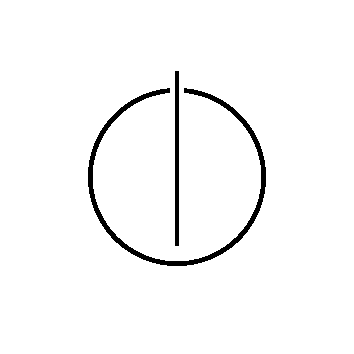
\includegraphics[width=4cm]{styles/informat.png}
  \end{figure}
  
  \end{center}
%	\clearemptydoublepage
%	
%	% The titlepage for the CAMP report document.
% Included by MAIN.TEX


%--------------------------------------------------
% The title page
%--------------------------------------------------

% correct BCOR - undo at the end !!!
\def\bcorcor{0.15cm}
\addtolength{\hoffset}{\bcorcor}

\thispagestyle{empty}

 \vspace{10mm}
\begin{center}
	       \oTUM{4cm}
	   
	   \vspace{5mm}     
	   \huge FAKULT{\"A}T F{\"U}R INFORMATIK\\ 
	   \vspace{0.5cm}
	 \large DER TECHNISCHEN UNIVERSIT{\"A}T M{\"U}NCHEN\\
        
	\end{center}
		

\vspace{10mm}
\begin{center}

   {\Large \doctype}

  \vspace{10mm}
  
  {\LARGE \title}\\
  
  
  \vspace{10mm}
  
  
  {\LARGE  \titleGer}\\
  
  
  \vspace{10mm}

    %\hfill
    \begin{tabular}{ll}
	   \Large Author:     & \Large \author \\[2mm]
	   \Large Supervisor:    & \Large \supervisor \\[2mm]				
	   \Large Advisor:	& \Large \advisor  \\[2mm]
	   \Large Date:       & \Large \date
	 \end{tabular}
	 
	 \vspace{5mm}
	 
	 \begin{figure}[h!]
  \centering
   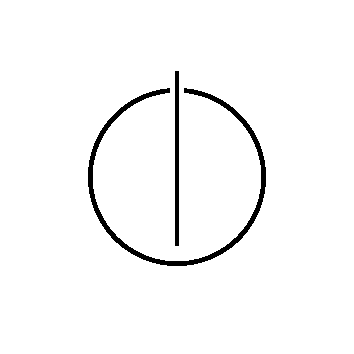
\includegraphics[width=4cm]{styles/informat.png}
  \end{figure}
   

\end{center}

% undo BCOR correction
\addtolength{\hoffset}{\bcorcor}
	
	
%	\input{components/cover_maschmeyer}
	\clearemptydoublepage
	
	% The titlepage for the CAMP report document.
% Included by MAIN.TEX


%--------------------------------------------------
% The title page
%--------------------------------------------------

% correct BCOR - undo at the end !!!
\def\bcorcor{0.15cm}
\addtolength{\hoffset}{\bcorcor}

\thispagestyle{empty}

 \vspace{10mm}
\begin{center}
	       \oTUM{4cm}
	   
	   \vspace{5mm}     
	   \huge FAKULT{\"A}T F{\"U}R INFORMATIK\\ 
	   \vspace{0.5cm}
	 \large DER TECHNISCHEN UNIVERSIT{\"A}T M{\"U}NCHEN\\
        
	\end{center}
		

\vspace{10mm}
\begin{center}

   {\Large \doctype}

  \vspace{10mm}
  
  {\LARGE \title}\\
  
  
  \vspace{10mm}
  
  
  {\LARGE  \titleGer}\\
  
  
  \vspace{10mm}

    %\hfill
    \begin{tabular}{ll}
	   \Large Author:     & \Large \author \\[2mm]
	   \Large Supervisor:    & \Large \supervisor \\[2mm]				
	   \Large Advisor:	& \Large \advisor  \\[2mm]
	   \Large Date:       & \Large \date
	 \end{tabular}
	 
	 \vspace{5mm}
	 
	 \begin{figure}[h!]
  \centering
   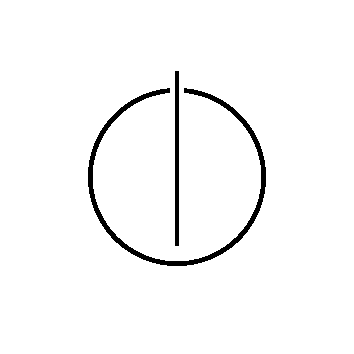
\includegraphics[width=4cm]{styles/informat.png}
  \end{figure}
   

\end{center}

% undo BCOR correction
\addtolength{\hoffset}{\bcorcor}
	
	
	\clearemptydoublepage


\thispagestyle{empty}
\selectlanguage{german}
	\vspace*{0.8\textheight}
	\noindent
	Ich versichere, dass ich diese Masterarbeit selbst{\"a}ndig verfasst und nur 
	die angegebenen \\Quellen und Hilfsmittel verwendet habe.
	
	\vspace{15mm}
	\noindent
	M{\"u}nchen, den \dateGer \hspace{5cm} \author
\selectlanguage{english}
\newpage
	
	\clearemptydoublepage
\phantomsection
\addcontentsline{toc}{chapter}{Acknowledgements}	


%\chapter*{Acknowledgements}

\vspace*{2cm}

\begin{center}
{\Large \bf Acknowledgments}
\end{center}

\vspace{1cm}




If someone contributed to the thesis... might be good to thank them here.
	
	% Abstract for the TUM report document
% Included by MAIN.TEX


\clearemptydoublepage
\phantomsection
\addcontentsline{toc}{chapter}{Abstract}	





\vspace*{2cm}
\begin{center}
{\Large \bf Abstract}
\end{center}
\vspace{1cm}

In this work we describe the process of adding the \cpppl\ support to \mbdp, an implementation of the
C programming language with extensions in a projectional language engineering environment, \jbmps. 
While implementing the \cpppl\ several well-known pitfalls of the language are taken into account
in an attempt to build a better C++ language flavor. Various analyses are implemented to improve
the programming experience for the end user. Lessons learned from this experience are described finally.
They include generalized principles, which could be used to improve a language while recreating it in a 
projectional language engineering environment; support of language modularity and extensibility  by \jbmps;
problems of building analyses and their complexity together with potential ways to resolve them in the future.

	\tableofcontents
  
  % \clearemptydoublepage
% 
% \phantomsection
% \addcontentsline{toc}{chapter}{Outline of the Thesis}
% 
% \begin{center}
% 	\huge{Outline of the Thesis}
% \end{center}
% 
% 
% 
% 
% %--------------------------------------------------------------------
% \section*{Part I: Introduction and Theory}
% 
% \noindent {\scshape Chapter 1: Introduction}  \vspace{1mm}
% 
% \noindent  This chapter presents an overview of the thesis and it purpose. Furthermore, it will discuss the sense of life in a very general approach.  \\
% 
% \noindent {\scshape Chapter 2: Theory}  \vspace{1mm}
% 
% \noindent  No thesis without theory.   \\
% 
% %--------------------------------------------------------------------
% \section*{Part II: The Real Work}
% 
% \noindent {\scshape Chapter 3: Overview}  \vspace{1mm}
% 
% \noindent  This chapter presents the requirements for the process.

	\mainmatter
	
	
		% ---------------------------------------------------------------------------
		%
		%Introduction and Background Theory
		%
		% ---------------------------------------------------------------------------
		\part[Introduction and Theory]{Introduction and Theory}
		\label{part:introAndBackgroundTheory}
		\chapter{Introduction}
\label{chapter:Introduction}

Here I introduce the main concepts and existing work, relevant to this \MT, as well as present the motivation for the topic.
 
\section{Projectional Editing}

This section compares the traditional approach to build textual editors for the program code with
the projectional approach, bringing up  motivation for the least.

\subsection{Traditional Approach}
Traditionally programming languages are used in a textual form in text files, forming programs.
However the textual nature is not typical for the structure of programs themselves, being rather low-level
representation of code. Parsers are used to construct so called abstract syntax trees (ASTs) from the textual 
program representation. ASTs are structures in memory, usually graph-alike, reminding sometimes control flow
graph, where nodes are different statements and edges are the ways control passes from one statement to the 
next one.

For the developer, using an editor, the degree to which the editor can support the development process is 
important. For this, the editor has to recognize the programming language construction and provide possible assistance.
Among such assistance can be code formatting, syntax validation, source code transformations (including refactoring support), code analyses and verification, 
source code generation and others. Many of these operation rely indeed on the higher than text level notions related to program such as method,
variable, statement. A good editor has to be aware of these higher level program structure.

Nowadays most of the editors work with text, and to provide assistance to programmer integrate with parser/compiler front-end 
for the programming language. This way to extract the program structure during editing is not perfect for several reasons.
First of all, the program being edited as text is not syntactically correct at every moment, being incomplete, for 
example. Under this circumstances the parsing front-end can not be successfully invoked and returns error messages
which are usually false-positive. Secondly, after minor editing of the code, usually the whole text file has to be
processed again. Such compiler calls are usually computationally expensive, they slow down, sometimes significantly, 
the performance of the developer machine. Various techniques exist to speed it up, including partial and pre- compilation,
but the problem is still relevant to large extent. 

Moreover, the textual nature of the code complicates certain operations additionally. As an example, we can take a refactoring
to rename a method. Every usage of the method, being renamed, has to be found and changed. To implement it correctly an editor
must take into account various possible name collisions, as well as presume a compilable state of the program to even start
the refactoring.

Not to mention the parsing problem itself. Parsing a program in a complex language like C++ is a difficult problem, it involves 
the need to resolve correctly scoping and typing, templates and related issues, work with pre-processor directives incorporated
in the code. In this regard different compilers treat C++ in a different way, creating dialects, which may represent obstacles for
the code to be purely cross-platform.

\cpp{Closing several blocks}{blocks}

The textual representation of program code, involves the need in formatting and preserving syntax. These both tasks, indeed,  
have nothing to do with program functionality, and addtionally load the developer, reducing productivity. As an example, here
I can mention the need to close several blocks ending at the same point correctly, indenting the closing brace symmetrically 
to opening one, and putting in the exact amount of braces. The \rl{blocks} demonstrates it in the last few lines.

\subsection{Projectional Approach}

Another approach which can be taken in the editor for a language is called projectional approach. Projectional editors
do not work with a low-level textual representation of a program, but rather with a higher level concept, ASTs.

Working with ASTs directly has several advantages over the conventional text editing. Firstly, all syntax errors are no longer
possible, as there is no syntax. Secondly, there is no need to format the code anyhow, since it is only typical for textual code.
Thirdly, all features, which in textual approach require parsing, can be implemented without parser, because AST is always known to the editor.

Projectional editors have to display somehow the AST to the developer, in order for him/her to work with it. Such visualization
of an AST is called ``projection'', giving a name to the editor class.

The model of code is stored as AST in the projectional editor. As in the Model-View-Controller pattern (\cite{GOF95}) the view for
the model can be implemented separately. Thus the code may look in a many different ways to the user. For example, the AST can be
visualized as a graph, similar to control flow graph. This visualization, however, is not always advantageous being sometimes not compact and
complicated to overview.

\ms{constructor}{Example projection of an AST, ``source code'' view}

One of the well-accepted way to visualize AST is buy visualizing its textual representation, as if it would was written 
as a code in the programming language, see \fig{constructor}. The statements in the projectional are only selected as whole.
There is now way to just select the ``while'' word for cut or copy, without selecting the condition and the block belonging
to the statement. This behavior represents the position of the condition and while-body in the AST as children of the while
statement. The statement can be selected all, only with children.

Additionally, each block delimiters are just a part of block visualization. They are organized in a proper way automatically,
and there is no way to delete or confuse them, as well as type them initially. Each closing brace is marked with the 
parent statement name (not a problem to implement such behavior in viewing AST), enhancing navigation through the AST's projection.

As one can see the projection to text in a projectional editor looks almost the same, as the conventional textual editor.
This can cause some confusion for the developer at first, as attempts to edit this textual visualization as a real text
will fail. Eventually, however, advantages of such visualization overwhelm the disadvantages. Among the benefits of the 
textual projection over text are quicker code construction after short learning, better way to select code fragments,
since not individual characters or lines, but rather AST nodes or groups of nodes are selected, plus all the advantages,
the projectional editing brings by itself, as discussed above.


\section{C++ in Projection}

The goal of this \MT\ is to research different aspects connected with implementation of the \cpppl\ in a projectional editor.
As a tool base for this \jbmps\ has been selected together with the based on it \mbdrp. This section overviews the technologies.

\subsection{\jbmps}

\jbmps\ stands for Jetbrains Meta Programming System. In this IDE-like software it is possible to develop domain specific languages.
The approach taken in the \jbmps\ is rather unique. One defines a language in it not through the canonical grammar approach, but instead
through defining so called concepts, and relationships between them similar to those in ER diagrams. A logical part of a language can be made 
a concept. Related to C++, class, method declaration, field declaration can be represented as a concept. 

Each concept can have children, which should be assigned with a role and cardinality. For example, the class concept can have children of method concept,
with a role called ``methods'', and cardinality 0..n.

Concepts can form hierarchies as classes normally do in object oriented programming languages. For this each concept should have a base concept (inheritance),
and can implement several interface concepts (interface implementation). Concepts can be abstract, for the use purely only in inheritance to create other 
non-abstract concepts with a common parent.

Each concept is described by several views on it. Among such views there are editor, behavior, constraints, type system, generator and few more views.

The editor view is designed to give a look for a concept, and a way to input it. This is where the projection of an AST node is defined. As editors 
are mostly defined to look like text, a program in the \cpppl implemented in MPS looks almost like a regular C++ code.

The behavior view, can be used to define certain behavioral methods for a concept. A concept is represented there similar to a java class, and
it is possible to define the methods in a Java-like language.

The constraints view can be used, to limit in a desirable way relationships the concept can have to other concepts.

The type system view is used mainly to define a type for each instance of a concept. The type is used later (for example, in the constraints), to 
determine suitability of the concept instance for a place, where it is used.

The generator view, as well as the textgen view, is used to define the way, the concept instance is going to be transformed when generation of the AST
is invoked by the MPS user. In general, the generation is needed in the end of the programming, to obtain the source code from the AST in a textual representation.
This textual representation is needed because all existing tools (like compilers) expect text code nowadays. It is worth mentioning that, in theory, one
could implement a compiler, which works directly from the AST in the editor, eliminating thus the need in generators to text.

The representation of a new language created in concepts and views to them, present a seamless approach to creating a new language with a projectional editor.
Thus \jbmps\ is a good suitable technology for the practical implementation of the \MT\ goal.

\subsection{mbeddr Project}

The \mbdrp\ represent mainly an implementation of the C programming language in the \jbmps\ environment. Having embedded systems
and software for them as a main focus, \mbdr\ provides certain language extensions to empower the programmer in the mentioned domain. 

Being a different language the \cpppl\ shares a lot of commonality with C. As \jbmps\ allows to some extent incremental language construction,
as the basis for the \cpppl\ implementation in \jbmps\ the \mbdrp\ was considered to be suitable. 

The use of \mbdr\, however, could not be purely incremental, and required some changes to the \mbdr\ itself. 
The changes were introduced however, in a way to make \mbdr\ simply more extensible, 
without creating a dedicated branch working as a basis for the \cpppl\ only.

\subsection{Motivation}

The selection of the topic for the \MT can be motivated in several ways.

At first, the author is not aware of any implementations of C++ editing in a projectional editor. The goal to research
such opportunities for one of the most complicated, traditionally highly text-oriented, object oriented languages is
new.

Secondly, extending the \mbdrp\ with the \cpppl\ has a practical interest for the \mbdrp\ users. Being comparatively lightweight,
the \cpppl\ supports object-oriented programming paradigms and more. It is thus of a high interest for embedded domain developers, using \mbdr,
to be able to have the \cpppl\ in the arsenal.

\subsection{Special Goals}

This work strives for some special goals, which are described below. These goals are targeted to either enhance
the user experience, or to make the implementation more technically elegant. All the goals have some influence on the implementation,
which is discussed in the following chapters, mentioning the goals.

\subsubsection{Special Goal 1: Embedded-Programming Domain}
\label{g1}

Being an extension for the \mbp\ the discussed in this \MT\ C++ implementation is following the general \mb\ goals. Among these goals are targeting
the embedded-programming domain.

\subsubsection{Special Goal 2: Enhancing the C++ Experience}
\label{g2}

It is hard to improve on one of the most beautiful programming languages. However, the usage of it can be improved
with special features of the editor, making the language, when possible, more supportive to the user. This can focus
towards an experience user-in-a-hurry, or to a novice, who is learning C++.

\subsubsection{Special Goal 3: Not-invasive Language Extending}
\label{g3}

The implementation of the \cpppl\ discussed in this work is an extension of the \mbp. 
Developing ``on top of'' the \mbp\ was not always possible through just the us of the \mbp\ 
as a layer of abstraction, one down to the layer, representing C++. However such a layered architecture
was desirable. Due to this sometimes modifications to the \mbp\ were required. 

The current goal consists of implementing all modifications to the \mbp\ in such a way, that only 
the C++ implementation has to be aware of the \mbp\ implementation details, but not the opposite! 
This is required to allow a separate development of the  \mbp\ without a look back to the C++ extension 
and still remaining the C++ extension working with a newer mbeddr versions. 

Such architecture is similar to layered architecture, but does not exactly represents one. The difference
is that the usage of the underlying \mbp\ can not be described only as the use of the interfaces, provided
by it. Sometimes there is simply no interfaces as such, and other ways have to be applied to make use of the
\mbp\ in a needed way. All the cases where the pure use of the mbeddr layer is not possible are discussed
separately in the work below. Thus, this work researches also the practical modularity and extensibility aspects of 
the language development and its support in \jbmps.
		
		
		%
		%% ---------------------------------------------------------------------------
		%%
		%% Fully Automated Calibration for Ultrasound
		%%
		%%% ---------------------------------------------------------------------------
		\part[The 2nd Part]{The Second Part}
		\label{part:secondP}
		\chapter{Structure}
\label{chapter:Structure}

Here the structure is going to be given

\section{Structure Itself}

Structure, now as a list

\begin{enumerate}
  
  \item Problem description
  
  \begin{enumerate}
    \item DSLs and Projectional Editing
    \item MBEDDR Project
    \item C++ Support in MBEDDR (motivation)
    \item Related Work
  \end{enumerate}
  
  \item Extending mbeddr with C++
    \begin{enumerate}
      \item Differences between C and C++
	\begin{enumerate}
	 \item Reference Type and Boolean Type
	 \item Modules Support
	 \item Object Oriented Approach Support
	\end{enumerate}
      
      
      
% Need in C++
% Challenge to implement
% MPS support
% Comprosises - trade of's



      
      \item Classes and Member Access Control
	\begin{enumerate}
	 \item Access Control in Class
	 \item Inheritance and Access Control
	 \item Friends	 
	\end{enumerate}

      
      \item Namespaces
	\begin{enumerate}
	 \item Namespace Resolution Operation
	 \item Member Search Strategy
	 \item Reenterability
	\end{enumerate}

      \item Operator Overloading
	\begin{enumerate}
	 \item Extension of Type System
	 \item ... More here ...
	\end{enumerate}

      
      
      \item Templates  
      \begin{enumerate}
       \item Textual Nature of Templates in C++
       \item Concepts
      \end{enumerate}

    
    \end{enumerate}
  
  \item Evaluation
  
  
  \item Conclusion 
  
\end{enumerate}
 



		
		
		% ---------------------------------------------------------------------------
		%
		% Appendix
		%
		% ---------------------------------------------------------------------------
		
		\part*{Appendix}
		\addcontentsline{toc}{part}{Appendix}
		
		\appendix %---------------------------------------
		
		\chapter{Detailed Descriptions}
%\section{Detailed Validation Results}
\label{chapter:DetailedDescriptions}
Here come the details that are not supposed to be in the regular text.
		
	


  \clearemptydoublepage
  
	\bibliography{bibliography/literature}
	
 
\end{document}